\documentclass[a4paper]{article}

\usepackage{amssymb, amsmath}
\usepackage[T1]{fontenc}
\usepackage[margin=0.6in]{geometry}
\usepackage{enumitem}
\usepackage{parskip}
\usepackage{lmodern}
\usepackage{array}
\usepackage{graphicx}

\title{\textbf{CS 520 Assignment 4: Colorization}}
\author{Raj Sundhar Ravichandran, Justin Chou, Vatsal Parikh}
\date{December 14, 2017}

\begin{document}

\maketitle
\section*{Source Code and Contributions}
Git Repository: https://github.com/jyqchou/AI-Colorization

\section*{Questions}

\begin{enumerate}
\item \textbf{Taking the shade values to be integers between 0 and 255, how many possible color values are there? How many possible grays? How many possible 3x3 gray pixel patches? Should a 3x3 pixel patch be enough information to guess the center color, or not enough?}

Since we are representing each color pixel in RGB values, there can be a possible of 256 values for each value in RGB. Therefore we get around 256*256*256 = 16777216 color values.
Again for gray pixels, if we represent the pixel value considering only that pixel, we get a possible of 256 ``gray'' values. This is not enough to encode RGB which has $256^3$ possible values and potentially lose significant data. By taking the 3x3 pixel patch, we have $256^9$ possible values; this contains more information than just the single pixel, but this still will not completely capture the true values of RGB correctly. Taking the 3x3 pixel would decrease the loss compared to just the single pixel.

\textbf{Under what contexts might it be enough to try to associate every shade of gray with a specific color, and color an image on a pixel by pixel basis?}

It may be enough to associate every shade of gray with a specific color if we are sure there are fewer than 256 total colors (RGB values) in the image. We could then theoretically have a perfect map of 1-256 gray values to 1-256 RGB values. If each RGB value in the image had its own unique gray value, then we would not need to analyze 3x3 gray pixel patches as the center pixel gray value would contain enough information to tell us what the true color is. 
\bigskip
\item \textbf{Why might it be a good idea to reduce the color-space or the patch-space, for instance by lumping certain shades of green together into one color? What should a good coloring algorithm do if it was fairly confident a pixel should be green or red, but certainly not blue?}

Reducing the color-space significantly reduces the time and space complexity of the mapping algorithm. Instead of having to differentiate between 10 different greens to map to, clustering the greens into one color effectively simplifies the problem to classification of just one green. If we are to consider each shades of color individually, we will have to encode $256^3$ colors into 256 gray values, which is not achievable without using encoding of some sort.

A good coloring algorithm, if it was fairly confident a pixel is NOT blue, should place a heavy weight on coloring the pixel with a low blue value, or the rgb value in which blue does not show up visually. Particularly, when calculating the distance between two RGB values, there should be a heavier weight on the blue component, as calculated errors between RGB values will be larger for large differences in the blue value.
\bigskip
\item \textbf{Describe your algorithm, and the design or parameter choices that went into your algorithm. What was your reasoning? What were the difficulties you had to overcome?}

Our algorithm begins by calculating 40 clusters of 9 parameters for the 3x3 matrices in input.csv over 40 iterations, and the same for color.csv. We selected these parameters by calculating error between our input.csv and color.csv with their respective final clusters. To measure how ``good'' our particular clusters were, we first defined error or distance functions.

For our gray clusters, we define our error as the distance between each corresponding pixel in the 3x3 matrix. We calculated the square difference between each pixel, and then we placed a weight of 0.8 on the center pixel difference, and the weight of 0.025 on the remaining 8 corner pixels differences. We reasoned that the center pixel gives us the most information to what the true color values are, and that the surrounding cells may comparatively have less of an influence on the true color. We then take the square root of the collective sum for our error. For our color clusters, we used a distance equation that better represented how ``far'' two colors are from each other visually, by placing a heavier weight on the green and blue components than the red difference:

\begin{equation}
  distance(color_1, color_2) = \sqrt{2(r_1-r_2)^2 + 4(g_1-g_2)^2 + 3(b_1-b_2)^2}
\end{equation}

With our Error functions defined, we then experimented with different values for our parameters. Below is a table of the calculated errors, with each cell corresponding to its \textbf{input gray error and then color error} for its respective parameters:

\begin{figure}[h!]
\centering
   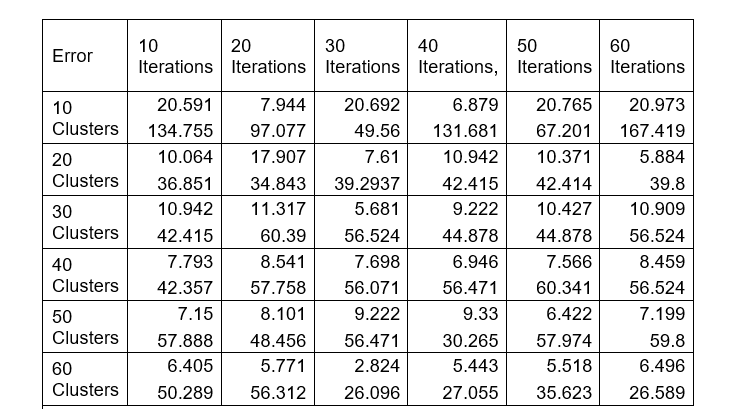
\includegraphics[width=0.7\textwidth]{table.png}
\caption{Calculated errors: input gray error and color error}\label{fig}
\end{figure}

We decided the ``elbow'' where the decrease in Error is the least is around 40 clusters with 40 iterations as we wished to select enough clusters to be able to fully represent the image, but reduced enough to simplify the problem into clusters. Similarly, we wanted to choose enough iterations to so our k-means algorithm would converge around the true clusters, but without doing extra iterations that necessary. The data we collected was also only after one trial each, so we could have improved our parameter selection if we gathered average Error and variance in Error for each N clusters and M iterations over a larger number of trials. 

Initially, we performed our k-means algorithm by randomly initializing 40 clusters. With this approach, we sometimes ended up with fewer than 40 final clusters as occasionally there were clusters that were matched with none of the observation points. We overcame this by initializing the 40 clusters to be random data observations.

Once we had our defined clusters for our input and color data, we then develop a mapping from each Black\&White Cluster to a particular Color Cluster. Our first approach was to simply iterate through each observation, and put each Gray Cluster as a key mapped to its corresponding Color Cluster in a hashmap. This approach placed a heavier influence on the data points at the end of our data, as previous key to value mappings were overwritten when a duplicate Gray Cluster was put as a key. We first decided to improve this by keeping track of every Color Cluster each Gray Cluster was mapped to, and formed a map to the Color Cluster that was observed the most frequently with a particular Gray Cluster.

Once this mapping is calculated, we can classify other 3x3 Black\&White matrices to their appropriate Black\&White Cluster and assign it the color based on the Color Cluster it maps to.
We, however, decided we could further improve our mapping with a neural network.

\textbf{Neural Networks Method in Python:}\\
Since the output of the above method was not efficient, we constructed neural network to better solve this problem. Our neural network consists of 9 input nodes, potentially, a node for each input value in 3*3 input black and white pixel. We constructed a hidden layer with 5 nodes in it. For each nodes in the initial layer, there is a connection to every other node in the second layer. In the final layer, we have 3 nodes, one for each in RGB. This again makes a fully connected structure, were each node in layer 2 is connected to each node in layer 3.

To this network, we loop through the given input.csv and pass each line of input at a time and also we give the corresponding line in color.csv as the expected network. We constructed the neural network with sigmoid functions, i.e., $1/(1+e^{(-x)})$

The weights in the first layer will be of the matrix form 9*5 and in the second layer as 5*3. These values are generated at random initially between -1 and +1. Once the output for first run is done, we calculate the error as (output - expected output). This error again is back propagated based on the weights of each link. After reading through all the data, we have potentially constructed a network with varying weights, which can predict a color value for any input black and white pixel intensity.

One main challenge we faced is, the error decreases to a certain limit and than again raises back. 
\begin{center}
\begin{tabular}{|c|c|}
\hline
Error at 10000th iteration & 232.460090641\\
\hline
Error at 20000th iteration & 82.0\\
\hline
Error at 30000th iteration & 54.666666667\\
\hline
Error at 40000th iteration & 97.666666667\\
\hline
Error at 50000th iteration & 114.0\\
\hline
\end{tabular}
\end{center}

To tackle this problem, we assumed by adding a regularization parameter or bias variable or implementing ReLU in convoluted neural network, would increase the efficacy of the model, predicting the colors more accurately. Ultimately, we were unable to minimize the error for our neural network, and the image produced using our mapping from the neural network was suboptimal. Our ``best'' image is using the most frequent mapping from Gray Clusters to Color Clusters, trained on our training data.


\bigskip
\item \textbf{How can you use the provided data to evaluate how good your coloring algorithm is? What kind of validation can you do? Quantify your algorithm's performance as best you can.}

We partition the input data into training, test, and validation data, where training consists of 80\% of the total input, test is 15\%, and validation is 5\%. We run our algorithm on the training data to establish our clusters and cluster mapping, and then we can apply this mapping to the test data and compare it to its corresponding values in color.csv. We are careful not to adjust our algorithm too much based on our results from our testing data to prevent overfitting. Once we are confident our algorithm colors beach photos well, we will apply the algorithm to our validation data and calculate the error from the corresponding values in color.csv

We can quantify our algorithm's performance by calculating the average error per pixel of our test or validation data set. For the purposes of this question, as a final evaluation of our algorithm, we calculate the error for our validation data set. This corresponds to observations 46451-48894. Since these are RGB values, we use our weighted ``visual'' difference calculation as noted in question 3, but also normalize the weights by a factor of 1/9 to calculate the average RGB value difference. 

We end up with the average error: 79.453. Thus, on average, our RGB pixel values are about 79.453/256 = 31.03\% of the 256 RGB value scale different. In terms of each RGB channel, our calculated differences are: Red Error = 79.816 or 31.17\%, Green Error = 32.517 or 12.70\%, Blue Error = 100.68 or 39.33\%\\
It is surprising to see that our Blue Error is the greatest, given we placed a heavier weight on it than we did on red. Visually, the Red Error has a smaller impact on the overall image, and our Blue Error can be explained by some portions of the image being ``too'' blue.

\bigskip
\item \textbf{Once you have trained your algorithm on input.csv and color.csv, use it to provide colors for each of the example patch data in data.csv. Submit the computed colors in a csv file, each row corresponding to the color of the corresponding row in data.csv.}

The color image constructed from data.csv based on the readings from input.csv and color.csv has been attached as Output.csv

\bigskip
\item \textbf{Where does your algorithm perform well, where does it perform poorly? How could you (with greater time and computational resources) improve its performance? What parameters or design decisions could you tweak? Would more data on more diverse images help or hinder your algorithm?}

Our algorithm performs well to categorize the gray pixels to blue shades correctly, but this blue also dominates the whole picture. We noticed that the partitioning of our data into training and test data may have affected the overall blue tint, as the initial 80\% of the data may consist of the pixels for the sky and water, whereas the last 20\% may include the colors of the beach. To check this, we ran one trial of training our program on the entire dataset, and the blue hue was slightly improved. Also the pictures are smudged along the edges of different colors. 

Data from more diverse images would certainly hinder the algorithm. As we train the algorithm on an image, it maps particular set of grey cell variations to a set of color data. So running this algorithm on a new unrelated data or training with diverse data would result in a color image that is visually off with totally unrelated colors.
\bigskip
\item \textbf{Do you think this is a reasonable approach to the problem? What would you change?}

The problem involves learning from a given set of data to then convert a new gray image to a color image. Therefore this can be done in supervised learning. Under supervised learning, one can consider doing linear regression, clustering, neural networks, or a combination of the three. 

Clustering is a reasonable first step as clustering reduces the complicated problem into a more simple one to solve. Where as we could have initially tackled the problem with a linear regression on the entire dataset without any preprocessing, our results would have a large amount of error due to the massive scale of the input $256^9$. Clustering allows us, to a certain degree, to eliminate variance in our data and capture the core properties of specific observations by treating ``close'' observations as the same, and effectively reduce input to 40 input values, and the output to 40 RGB values. 

Once we have preprocessed the data into clusters, neural networks is an effective method to map the input clusters to the color clusters. When building a neural network from the defined clusters, in theory we should be able to come up with an accurate function to map any 3x3 matrix to an RGB matrix; however, we couldn't re-propagate the errors back into the system properly. Since we decided to move on with the neural networks, we didn'
t have enough time to decode the issue further, so our ``best'' algorithm maps the Gray Clusters to Color Clusters based on the most frequent mappings within our training data. 

Upon another trial, I think it would be worth investigating the averaging function for RGB. While for gray pixels the arithmetic mean of gray pixel values corresponds to the ``visual'' mean, this is not the case for RGB. While our calculated Color Clusters converge to a color with the ``lowest distance'', calculating the arithmetic average of the RGB may not allow us to reach a true convergence of average color. We may have more accurate color clustering if we converted RGB to the Lab color space, computed the average Lab values, and then converted that back to RGb. Furthermore, many of our issues came from our neural network. For the future, if we can simplify our activation function for our neural network, our gradient would be easier to calculate for updating the weights of our branches. In both instances, we were able to detect when our ``error'' was large, and we knew to minimize the error through additional iterations of clustering and adjusting weights, but we had difficulty actually calculating those true mean clusters and weights.
\bigskip
\item \textbf{What would happen if you tried to color a grayscale image of a tiger, after training your algorithm on pictures of palm trees?}

Our algorithm would attempt to color the tiger as if it were an image of palm trees. Namely, since the algorithm is trained to color beach, i.e. detect and color skies and the ocean blue, sand beige, the clouds white and leaves green, the algorithm would similarly interpret 3x3 pixel matrices of the tiger and color them as if they were 3x3 pixel matrices of the sky, ocean, sand, clouds, or leaves. We would then get an image of the tiger that is colored blue, beige, white, and green in areas the algorithm believes to similar to areas of the sky, ocean, sand, clouds, or leaves, most likely in a manner that does not visually make much sense to us. We would need to train our data on other images of tigers before coloring them.
\end{enumerate}


\section*{Bonus}
\textbf{Write your program to take in an image, convert it to grayscale, train your algorithm, and then use the algorithm to color example grayscale images. How does your algorithm do, visually?}
\begin{figure}[h!]
\centering
   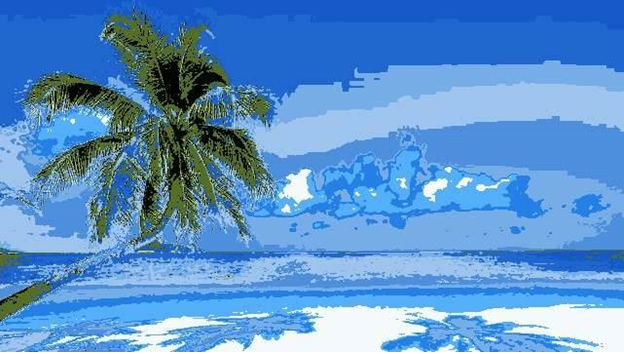
\includegraphics[width=0.7\textwidth]{output_image.png}
\caption{Output image}\label{fig}
\end{figure}

There is blue where we expect there to be blue, such as in the sky and in the water, but it also bleeds into other areas such as the palm tree and sand. Similarly, we have some white in our clouds, but we also have white on the beach, and green in the trunk of the tree. It seems that we do not correctly map any Gray Cluster to Colored Clusters of brown (such as in the trunks) or beige (in the sand) correctly.
\end{document}